This section defines the top-level logical view of the design and describes the detail architectural strategy for the RV8 work cell system flow. Three separate layers make up the structure of the system: input, processing, and output. With the help of these layers, which are all essential to the system, the robot is able to carry out dynamic tasks that are dependent on the processing of sensor data. A high-level block diagram that shows the connections and interactions between different layers is included in this part to provide readers a thorough understanding of the architecture of the entire system. A robotic system's input layer, which makes use of sensors like a gate sensor and an E-stop is essential for task execution. E-stops offer an emergency shutdown signal that allows the system to be stopped right away. The robot arm's speed is controlled by the Gate sensor, which also communicates with the controller to find out the cage gate's present state. Efficiency and safety are prioritized in this design, which allows the robot to respond and adapt to a variety of scenarios while integrating security features like gate status monitoring and emergency stops. With the integration of sensors will perform the operation such as splashing multi-color paint to the desire target with great level of precision. PC and the trigger switch will be inter-connected to the PC to perform the necessary communication to perform the given task.  

\begin{figure}[h!]
	\centering
 	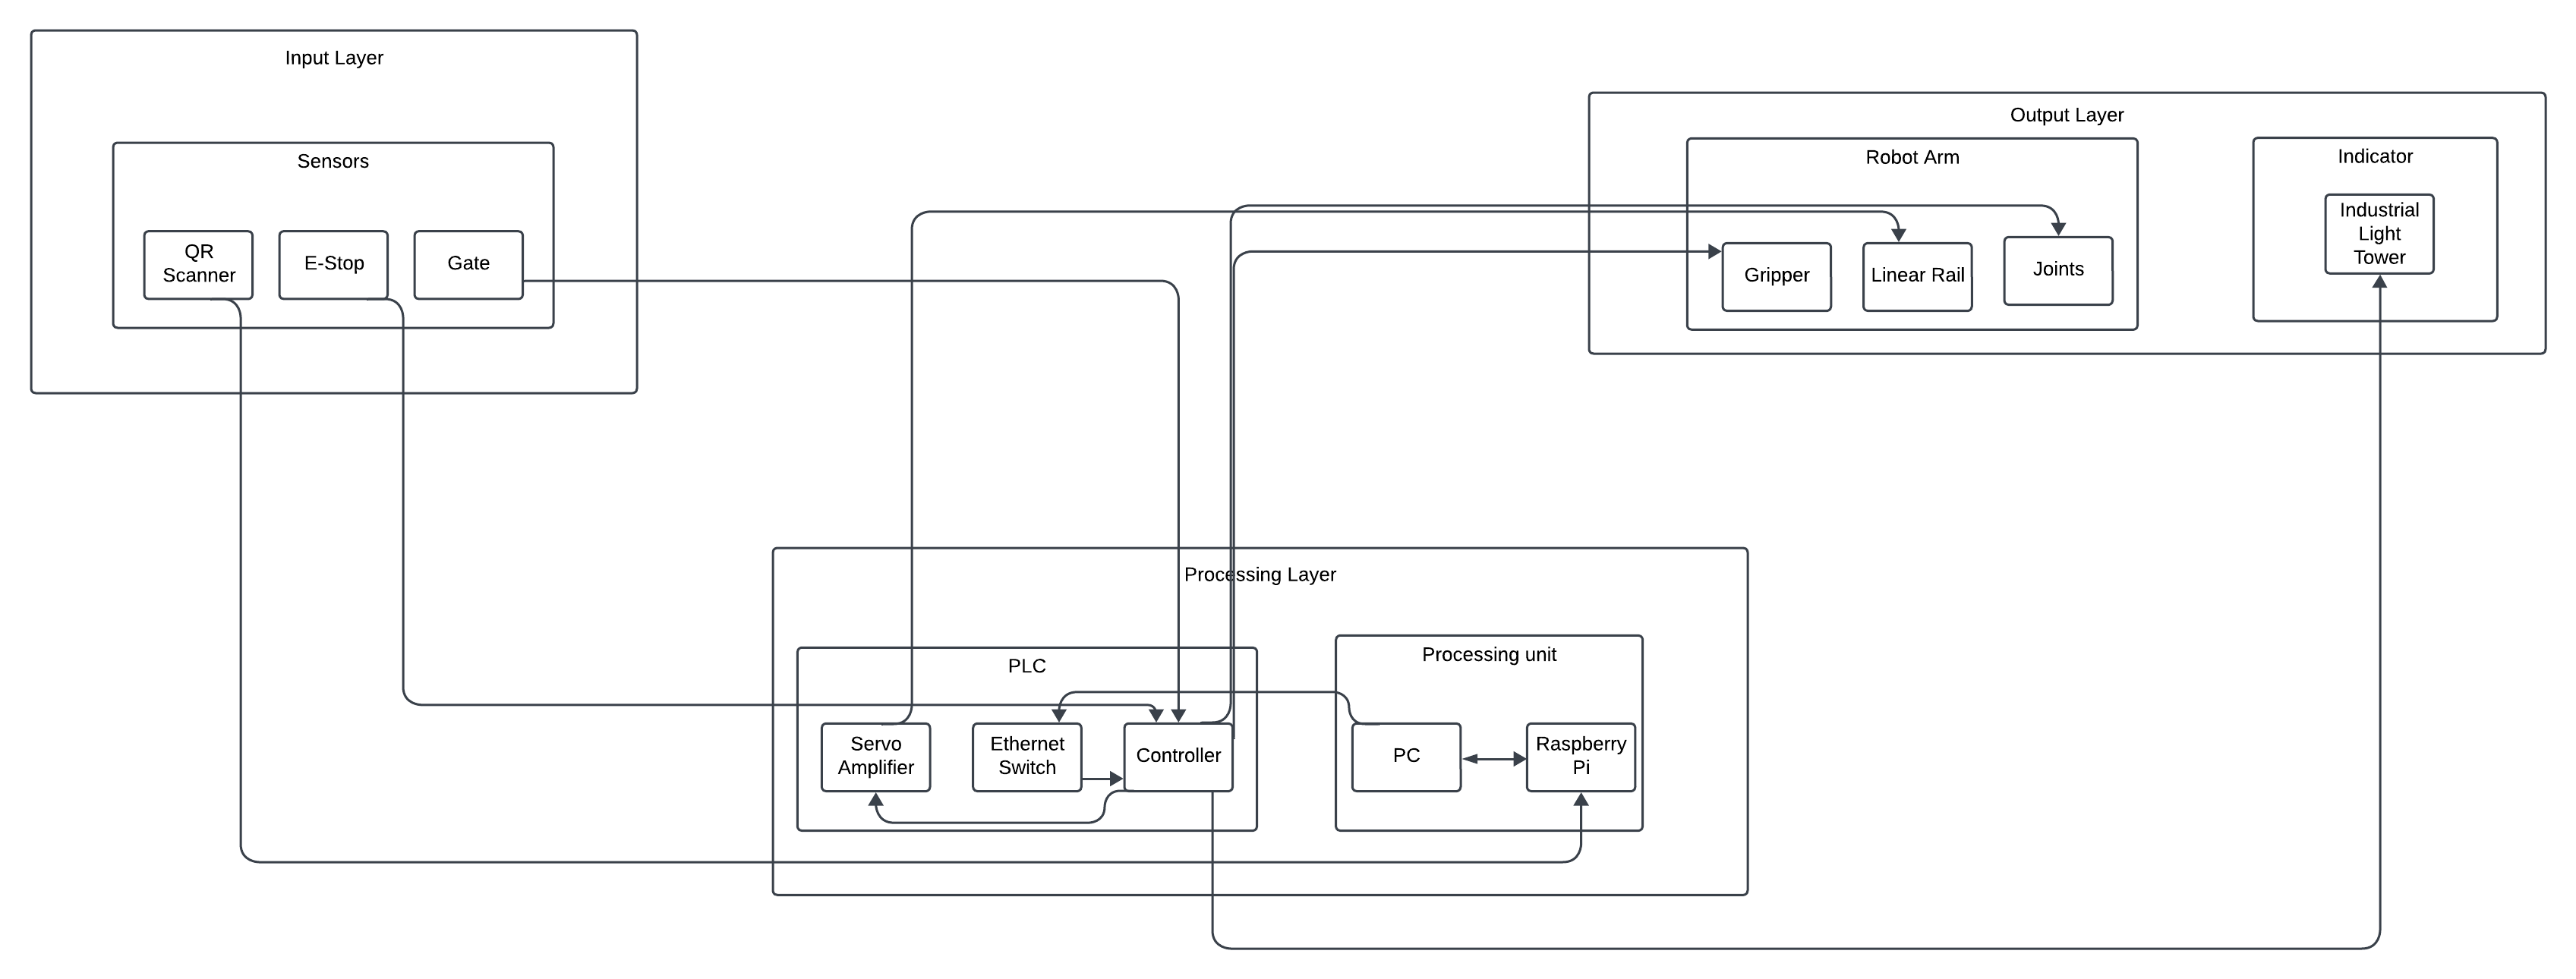
\includegraphics[width=1\textwidth]{images/system_subystem.png}
 \caption{System architecture}
\end{figure}
